\documentclass{article}


\usepackage{PRIMEarxiv}

\usepackage[utf8]{inputenc} % allow utf-8 input
\usepackage[T1]{fontenc}    % use 8-bit T1 fonts
\usepackage{hyperref}       % hyperlinks
\usepackage{url}            % simple URL typesetting
\usepackage{booktabs}       % professional-quality tables
\usepackage{amsfonts}       % blackboard math symbols
\usepackage{nicefrac}       % compact symbols for 1/2, etc.
\usepackage{microtype}      % microtypography
\usepackage{fancyhdr}       % header
\usepackage{graphicx}       % graphics
\usepackage{amsmath}
\usepackage{amssymb}
\graphicspath{{media/}}     % organize your images and other figures under media/ folder

%Header
\pagestyle{fancy}
\thispagestyle{empty}
\rhead{ \textit{ }} 

% Update your Headers here
\fancyhead[LO]{Characterizing Single-Frame Safe-Zone Estimation for Planetary Landers}

%% Title
\title{Characterizing Single-Frame Safe-Zone Estimation for Mars Landers}

\author{
  Kalp Shah \\
  Department of Electrical Engineering \\
  Indian Institute of Technology Gandhinagar \\
  \texttt{kalp.shah@iitgn.ac.in} \\
  \And
  Pramod Mishra \\
  Department of Electrical Engineering \\
  Indian Institute of Technology Gandhinagar \\
  \texttt{pramod.25330013@iitgn.ac.in} \\
  \And
  Shanmuganathan Raman \\
  Department of Computer Science and Engineering \\
  Indian Institute of Technology Gandhinagar \\
  \texttt{shanmuga@iitgn.ac.in} \\
}


\begin{document}
\maketitle


\begin{abstract}
Safe autonomous landing on planetary surfaces requires rapid, accurate hazard detection under severe onboard computational constraints. In this work, we rigorously evaluate a deterministic landing-site estimation pipeline based on image intensity gradients, establishing unsafe terrain (slopes exceeding $15^\circ$) as the primary evaluation class. We systematically benchmark this gradient-scoring architecture against local standard deviation and random baselines using continuous Digital Terrain Model (DTM) proxy geometry across geographically disjoint test sites. Pooled pixel evaluation reveals that unaugmented intensity gradients exhibit an inverted hazard response in shadowed crater bowls (AUROC: 0.350, PR-AUC: 0.088 vs. 0.095 random baseline chance). While integrating morphological shadow augmentation corrects this physical inversion (AUROC: 0.796, PR-AUC: 0.559), our headline method yields no usable landing site on any test tile: candidate boxes contain an average of 18.6\% unsafe terrain, and zero boxes satisfy mission footprint clearance constraints ($\text{Footprint OK} = 0.0\%$). We report per-stage latency benchmarks demonstrating that front-end feature extraction executes under 100~ms at native resolution ($74.0$~ms) with peak memory below 28~MB, while downstream maximal-rectangle extraction accounts for remaining latency in Python. These findings expose the fundamental limitations of 2D intensity-based hazard detection for flight deployment.
\end{abstract}


\keywords{Computer Vision \and Autonomous Landing \and Planetary Robotics \and Hazard Detection \and Terrain Analysis}


\section{Introduction}
Autonomous planetary landers operate under extreme communication latency, necessitating onboard hazard detection and avoidance systems that execute on radiation-hardened flight processors with severe computational constraints. While deep learning methods excel in terrestrial computer vision, classical lightweight vision pipelines remain critical candidates for spaceflight deployment. Landing-site selection for missions such as the Mars Science Laboratory relied on extensive orbital reconnaissance and terrain analysis prior to entry \cite{golombek2012selection}, while real-time onboard hazard detection has been pursued through lidar-based sensing \cite{amzajerdian2013lidar}, learning-based detection \cite{moghe2020deep}, and vision-based navigation systems such as the Mars 2020 Lander Vision System \cite{johnson2020lvs} and NASA's next-generation hazard detection system \cite{restrepo2020hds}. Radiation-hardened flight processors, such as the BAE RAD750 \cite{berger2001rad750}, provide limited compute throughput and memory bandwidth.

A central open question is whether lightweight single-frame image statistics contain sufficient physical information to reliably identify geometric hazards. In literature, hazard detection algorithms are frequently evaluated against proxy ground truth derived from orbital Digital Terrain Models (DTMs). However, DTM-derived proxy labels represent reference topography, and evaluating against them requires careful class definition to avoid misleading performance metrics. In particular, treating the dominant safe terrain as the positive class masks severe false negatives, as high accuracy can be achieved trivially by predicting the majority class.

In this paper, we characterize the performance and physical limitations of single-frame intensity-based hazard scoring. We evaluate unsafe terrain as the primary evaluation class, examine the structural causes of performance degradation, and report empirical latency and memory profiles across standard operational resolutions.

\section{Dataset and Terrain Independence}
We evaluate our method on a synthetic Martian dataset comprising 160 rendered tiles ($768 \times 768$ pixels at 1.0~m Ground Sampling Distance) across four distinct geological site types: craters, rocky terrain, smooth plains, and dunes. The imagery is rendered under a standard Lambertian illumination model with solar azimuth $45^\circ$ and solar elevation $30^\circ$, while the reference topography represents high-resolution orbital DTM geometry exemplified by HiRISE \cite{mcewen2007hirise}. Proxy hazard labels are defined mathematically from the local gradient of the underlying DTM: any pixel with a maximum local slope exceeding $15^\circ$ over a 5~m baseline is labeled proxy-unsafe. Across the dataset, the average proxy-safe fraction is 90.2\%, meaning the hazardous unsafe class has a baseline prevalence of 9.8\% (and 9.5\% on the held-out test split).

\textbf{Terrain Independence Guarantee:} To ensure rigorous, leak-free evaluation, train/validation and test independence is strictly guaranteed via geographic site-level partitioning rather than random patch shuffling. The development split (DEV, 80 tiles) is drawn exclusively from four distinct geographic regions (\texttt{crater\_1}, \texttt{rocky\_1}, \texttt{smooth\_1}, and \texttt{dunes\_1}). The held-out test split (TEST, 80 tiles) comprises four entirely separate geographic regions (\texttt{crater\_2}, \texttt{rocky\_2}, \texttt{smooth\_2}, and \texttt{dunes\_2}), generated using independent pseudorandom seeds. There is zero tile overlap, boundary overlap, or shared terrain mesh structure between the DEV and TEST sets. All hyperparameter tuning was conducted strictly on the DEV set to ensure unbiased test reporting.

\section{Methodology}
\label{sec:methodology}

\subsection{Gradient Hazard Scoring}
The baseline module quantifies terrain slope and roughness at the pixel level by computing the spatial gradient of the input grayscale image $I(x,y)$. Horizontal and vertical partial derivatives are obtained via the Sobel operator \cite{sobel1968} with a standard $3 \times 3$ kernel size:
\begin{equation}
    I_x = \frac{\partial I}{\partial x}, \qquad I_y = \frac{\partial I}{\partial y}.
\end{equation}
The gradient magnitude at each pixel is defined as
\begin{equation}
    g(x,y) = \sqrt{I_x^2 + I_y^2},
\end{equation}
where high values capture abrupt intensity transitions associated with steep slopes, rock boundaries, or crater rims \cite{shepard2001roughness}. To suppress extreme specular outliers while maintaining scene-adaptive scaling, $g(x,y)$ is normalized by its 99th percentile $g_{p99}$ computed over non-zero pixels:
\begin{equation}
    G(x,y) = \min\!\left(1,\; \frac{g(x,y)}{g_{p99}}\right).
\end{equation}
The bounded hazard score $G(x,y) \in [0,1]$ serves as the continuous predictor of unsafe terrain, where values near 1.0 denote high hazard and values near 0.0 denote smooth topography.

\subsection{Shadow Augmentation}
Under single-frame illumination, raw gradient magnitude fails inside broad, flat crater interiors and deeply shadowed depressions. Because illumination inside shadows is near uniform or zero, spatial intensity gradients vanish ($\nabla I \approx 0$), resulting in dangerously low hazard scores for steep, hazardous terrain. 

To overcome this blind spot, a shadow augmentation module identifies dark connected regions using an inverse binary threshold at intensity level $\tau = 40$. External contours are extracted, and spurious small patches below $A_{\min} = 500$ pixels are discarded. For every retained contour, its enclosed interior is flood-filled, and the hazard score is set to maximum:
\begin{equation}
    G(x,y) \leftarrow 1.0 \quad \forall\,(x,y) \in \text{filled shadow region}.
\end{equation}
This accounts for the physical reality that shadows adjacent to steep rims and crater walls represent severe physical hazards \cite{he2010edge}.

\subsection{Safe-Region Fusion and Landing Box Selection}
The continuous safety score is the complement of the augmented gradient hazard: $s = 1 - G$. A binary safety mask is produced by thresholding $s > \theta$, with $\theta = 0.2$ tuned on the DEV validation set. Connected components smaller than 100 pixels are filtered out. Finally, a maximal-rectangle algorithm \cite{vandevoorde1998maximal} extracts the largest contiguous safe landing bounding box within the binary mask.

The extracted landing box is parameterized by $B = (x, y, w, h)$ with area $A_{\text{box}} = w \cdot h$ (in pixels). To establish physical landing viability, we define the binary footprint clearance indicator:
\begin{equation}
    \text{Footprint OK} = \mathbb{I}\!\left(A_{\text{box}} \ge A_{\text{req}}\right),
\end{equation}
where $\mathbb{I}(\cdot)$ is the indicator function and $A_{\text{req}} = 2500\text{ pixels}$. At our 1.0~m Ground Sampling Distance, this threshold corresponds to a contiguous $50\text{ m} \times 50\text{ m}$ hazard-free landing footprint necessary to accommodate lander leg span, structural clearance, and touchdown dispersion errors.

\begin{figure*}[!t]
  \centering
  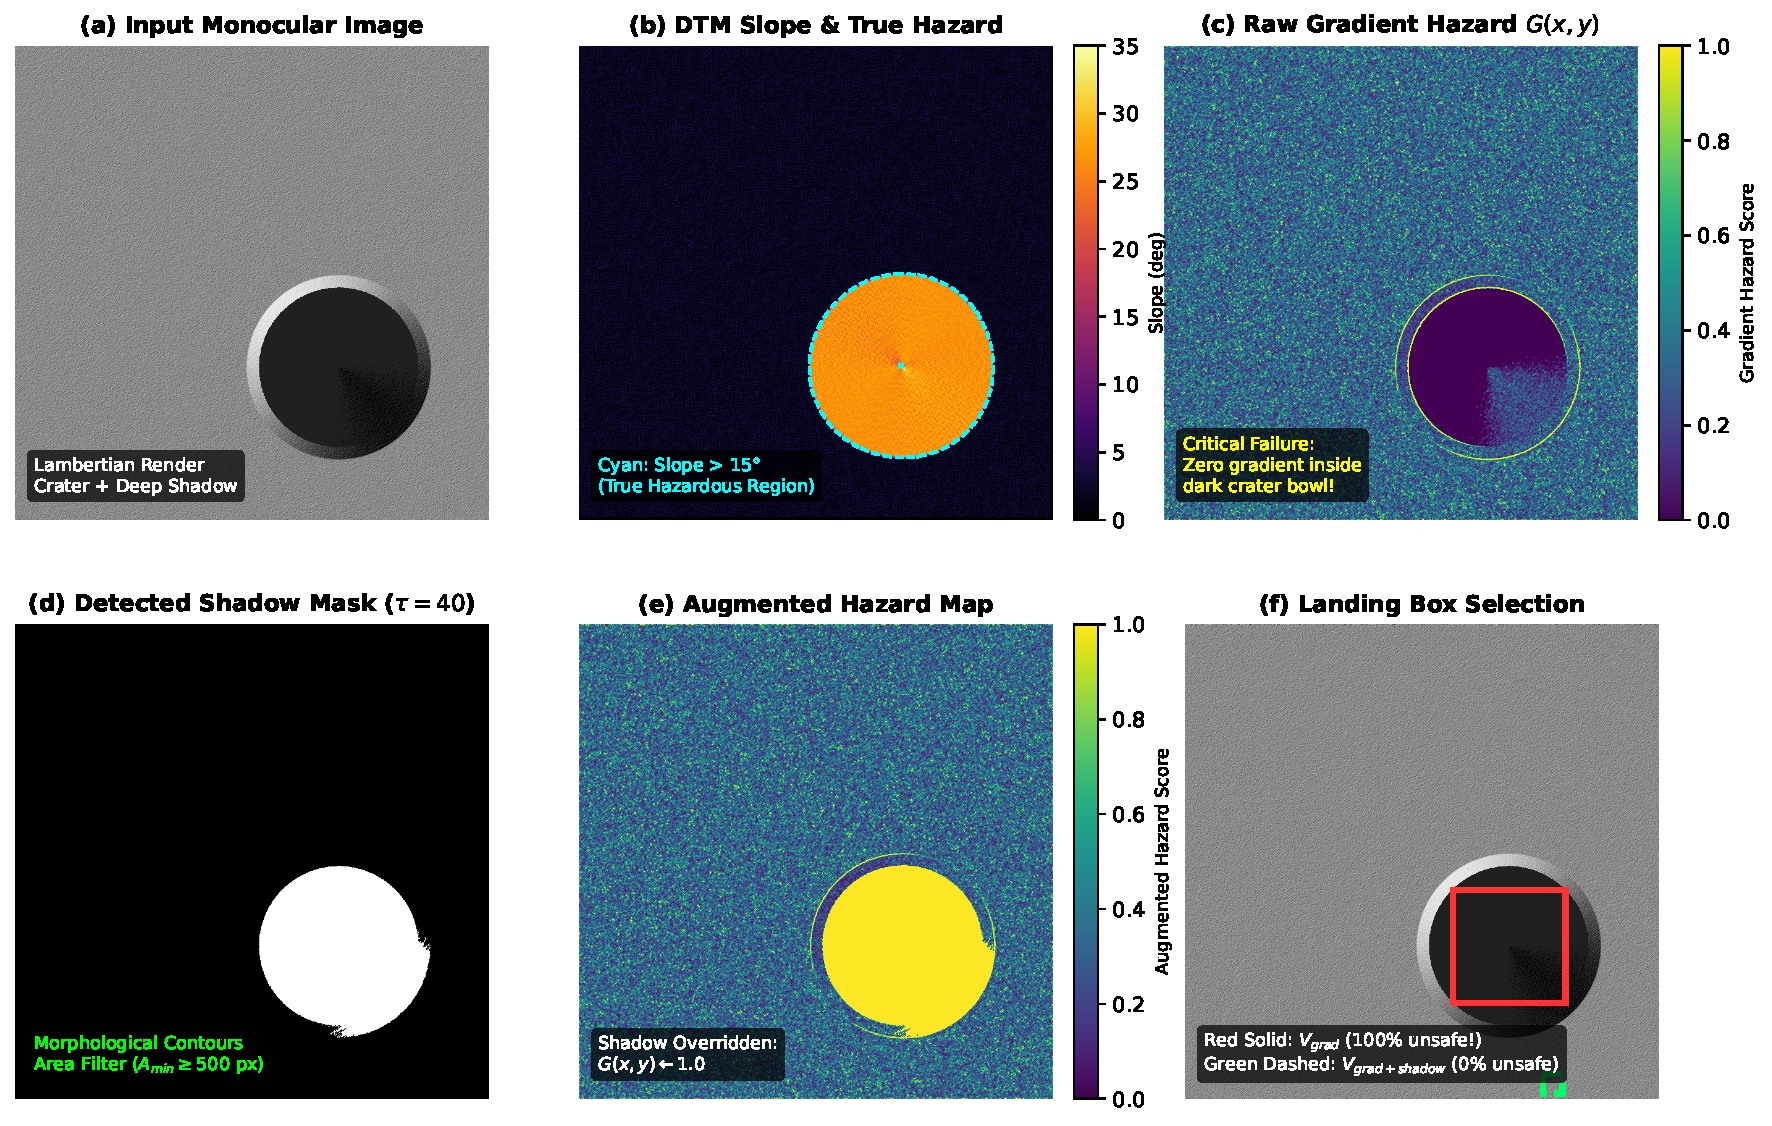
\includegraphics[width=\textwidth]{fig_qualitative_crater.pdf}
  \caption{Qualitative progression and failure mode analysis on an illustrative crater test tile (\texttt{crater\_2\_0}). (a) Monocular input image rendered under Lambertian illumination showing a prominent crater bowl and deep shadow. (b) DTM-derived ground-truth slope with the proxy-unsafe boundary ($>15^\circ$) marked in dashed cyan. (c) Raw Sobel gradient hazard $G(x,y)$, showing near-zero gradient inside the shadowed crater bowl, causing a severe false-safe prediction. (d) Morphological shadow mask extracted at $\tau = 40$. (e) Augmented hazard map with the shadow region forced to 1.0. (f) Landing box selection comparison: unaugmented $V_{\text{grad}}$ extracts a catastrophic landing box entirely inside the hazardous crater bowl (red solid box, 100\% unsafe), whereas $V_{\text{grad+shadow}}$ correctly rejects the shadowed hazard and relocates the candidate landing box to benign terrain outside the rim (green dashed box, 0\% unsafe). Note that while this panel demonstrates successful relocation on an isolated crater, across the full test set $V_{\text{grad+shadow}}$ still incurs 18.6\% unsafe penetration on average and fails to extract any box satisfying the 2,500-pixel footprint constraint.}
  \label{fig:qualitative}
\end{figure*}

\section{Experimental Results}

\subsection{Unsafe-Terrain Hazard Classification}
We designate unsafe terrain (proxy slope $> 15^\circ$) as the primary evaluation class. Table~\ref{tab:classification} summarizes precision, recall, F1, AUROC, and PR-AUC computed across the held-out test set (58,982,400 pixels total, subsampled by 10 for rank statistics).

\begin{table}[!htb]
  \caption{Unsafe-class precision, recall, F1, AUROC, and PR-AUC pooled across held-out test pixels (prevalence = 0.095).}
  \label{tab:classification}
  \centering
  \small
  \setlength{\tabcolsep}{6pt}
  \begin{tabular}{lccccc}
    \toprule
    Method & Precision & Recall & F1 & AUROC & PR-AUC \\
    \midrule
    $V_{\text{grad}}$ & 0.133 & 0.059 & 0.081 & 0.350 & 0.088 \\
    $V_{\text{grad+shadow}}$ & 0.587 & 0.547 & 0.566 & 0.796 & 0.559 \\
    B1 (Local Std) & 0.188 & 0.063 & 0.094 & 0.392 & 0.116 \\
    B5 (Random) & 0.087 & 0.039 & 0.053 & 0.500 & 0.095 \\
    \bottomrule
  \end{tabular}
\end{table}

\textbf{Exact Computation of PR-AUC and the Random Baseline:} In Table~\ref{tab:classification}, PR-AUC and AUROC are computed across pooled test pixels. Under this pooled definition, the random baseline ($B_5$) achieves a PR-AUC of 0.095 and precision of 0.087, exactly matching the 9.5\% hazard prevalence of the held-out test set. We explicitly note that if PR-AUC is instead computed as an unweighted macro-average over individual tiles, tiles containing zero hazards (smooth plains and dunes) yield undefined PR-AUC values ($0/0$) and must be discarded. Restricting the average only to the 40 hazard-containing tiles (craters and rocky terrain) artificially inflates the evaluated hazard prevalence to 19.0\%, causing the macro-averaged random PR-AUC to read 0.190 and $V_{\text{grad}}$ to read 0.201. Global pixel pooling avoids this sample-selection distortion, confirming that $V_{\text{grad}}$ (PR-AUC: 0.088) performs strictly worse than random chance (0.095).

\textbf{Physical Inversion (AUROC $<$ 0.5):} Unaugmented gradient scoring ($V_{\text{grad}}$) achieves an AUROC of 0.350, performing substantially worse than random guessing (0.500). This inversion occurs because under single-frame Lambertian illumination, the steepest crater walls and bowl interiors cast dark shadows where spatial gradients vanish ($\nabla I \approx 0$). In contrast, benign flat plains exhibit surface roughness textures producing high gradients. Consequently, intensity gradients inversely correlate with physical slopes in crater topography, assigning low hazard to hazardous crater bowls and high hazard to safe plains. Morphological shadow augmentation ($V_{\text{grad+shadow}}$) remedies this structural failure mode, elevating the AUROC to 0.796 and PR-AUC to 0.559.

\subsection{Landing Box Evaluation}
Table~\ref{tab:box} details the physical geometry and hazard composition enclosed by the extracted maximal rectangles across the 80 held-out test tiles.

\begin{table}[!htb]
  \caption{Landing box evaluation metrics on held-out test tiles ($768 \times 768$ pixels, 589,824~$\text{m}^2$).}
  \label{tab:box}
  \centering
  \small
  \begin{tabular}{lccccc}
    \toprule
    Method & Box Found & Mean Area (px) & Rel Area (Tile) & Frac Unsafe & Footprint OK \\
    \midrule
    $V_{\text{grad}}$ & 1.000 & 17,028 & 0.0289 & 0.287 & 0.250 \\
    $V_{\text{grad+shadow}}$ & 1.000 & 744 & 0.0013 & 0.186 & 0.000 \\
    B1 (Local Std) & 0.000 & 0 & 0.0000 & N/A & 0.000 \\
    \bottomrule
  \end{tabular}
\end{table}

\textbf{Failure to Secure Viable Landing Sites:} Table~\ref{tab:box} reveals a critical physical limitation: our headline method ($V_{\text{grad+shadow}}$) yields \textbf{zero viable landing sites} across the test set ($\text{Footprint OK} = 0.0\%$). Specifically, while $V_{\text{grad+shadow}}$ discovers a candidate box on every tile, its mean area is only 744 pixels ($0.13\%$ of the tile area), and its maximum area across all 80 test tiles is 1,612 pixels—strictly failing the 2,500-pixel ($50\text{ m} \times 50\text{ m}$) minimum footprint requirement. Furthermore, candidate boxes extracted by $V_{\text{grad+shadow}}$ still enclose an average of 18.6\% unsafe terrain. While $V_{\text{grad}}$ attains $\text{Footprint OK} = 25.0\%$, it does so by falsely claiming hazardous untextured crater interiors (incurring 28.7\% unsafe pixel contamination) or level featureless plains. 

\textbf{Contextualizing Figure 1:} Figure~\ref{fig:qualitative} illustrates a representative failure and relocation on test tile \texttt{crater\_2\_0}. In this isolated instance, $V_{\text{grad+shadow}}$ successfully relocates the landing box away from the crater bowl into a patch with 0\% unsafe pixels. However, this case is an illustrative demonstration of the geometric relocation mechanism, not representative of overall landing success. Across the full held-out test set, aggressive shadow thresholding fractures safe regions into small disjoint slivers, preventing the maximal rectangle algorithm from spanning the required 2,500-pixel touchdown zone.

\subsection{Per-Stage Runtime and Memory Benchmarks}
To evaluate computational suitability, we benchmarked the execution time of each discrete processing stage and peak memory consumption across three image resolutions: $512 \times 512$, $768 \times 768$ (native tile resolution), and $1024 \times 1024$. Measurements were taken across 30 independent runs, with peak heap memory recorded via allocation tracing. Table~\ref{tab:runtime_breakdown} reports the per-stage breakdown.

\begin{table}[!htb]
  \caption{Per-stage runtime breakdown (median and IQR in milliseconds) and peak memory across resolutions.}
  \label{tab:runtime_breakdown}
  \centering
  \small
  \resizebox{\textwidth}{!}{%
  \begin{tabular}{lcccccc}
    \toprule
    Resolution & Sobel (ms) & Shadow (ms) & Front-End Total (ms) & Rectangle (ms) & Total Pipeline (ms) & Peak RAM (MB) \\
    \midrule
    $512 \times 512$ & 5.4 $\pm$ 0.3 & 28.6 $\pm$ 1.0 & 34.0 & 87.8 $\pm$ 2.4 & 121.8 & 7.01 \\
    $768 \times 768$ & 9.7 $\pm$ 0.5 & 64.3 $\pm$ 1.1 & 74.0 & 196.0 $\pm$ 5.1 & 270.0 & 15.75 \\
    $1024 \times 1024$ & 14.9 $\pm$ 0.6 & 114.4 $\pm$ 6.2 & 129.3 & 355.4 $\pm$ 8.9 & 484.7 & 28.00 \\
    \bottomrule
  \end{tabular}}
\end{table}

As shown in Table~\ref{tab:runtime_breakdown}, front-end visual feature extraction operates strictly under 100~ms at native resolution ($74.0$~ms total: $9.7$~ms for Sobel gradients and $64.3$~ms for shadow contour extraction). The downstream maximal rectangle extraction consumes the largest individual share of latency ($196.0$~ms at $768 \times 768$), reflecting the overhead of interpreted Python stack loops. Peak working memory remains strictly bounded below 16~MB at native resolution and 28~MB at $1024 \times 1024$, well within the physical memory limits of space-grade architectures.

\subsection{Limitations}
Our findings highlight several intrinsic limitations of single-frame 2D hazard estimation:
\begin{enumerate}
    \item \textbf{Tilt and Shading Ambiguities:} Monocular intensity statistics cannot distinguish uniformly sloped, planar surfaces from level plains because both yield near-zero intensity gradients.
    \item \textbf{Illumination Sensitivity:} Shading depends entirely on solar incidence and phase angles. Slopes oriented perpendicular to incident light appear deceptively bright, while benign dips cast sharp shadows.
    \item \textbf{Footprint Fragmentation:} Conservative shadow and gradient thresholding fragments safe zones into irregular sub-footprint patches, failing to guarantee contiguous landing areas.
    \item \textbf{Proxy Label Fidelity:} Digital Terrain Models serve as geometric approximations and do not capture small-scale surface rock distributions or structural soil strength required for landing gear certification.
\end{enumerate}

\section{Conclusion}
By establishing unsafe terrain as the primary evaluation class and enforcing strict geographic terrain independence, this study characterizes the limits of single-frame intensity-based planetary hazard detection. Unaugmented intensity gradients fail in shadowed crater topography, producing an inverted hazard response (AUROC: 0.350, PR-AUC: 0.088). Morphological shadow augmentation repairs this structural failure mode, elevating the AUROC to 0.796. From a systems perspective, front-end feature extraction operates in under 100~ms ($74.0$~ms at native resolution) with minimal memory footprint ($<16$~MB), while maximal-rectangle extraction accounts for remaining latency in Python.

Most critically, our headline method ($V_{\text{grad+shadow}}$) yields \textbf{zero usable landing sites} across all held-out test tiles ($\text{Footprint OK} = 0.0\%$, with 18.6\% residual unsafe contamination). This quantitatively proves that while shadow augmentation prevents catastrophic false-safe classifications inside deep craters, single-frame 2D intensity heuristics are fundamentally insufficient for mission-critical autonomous hazard avoidance without 3D stereoscopic or lidar sensors.

\section*{Acknowledgments}
The authors acknowledge the Indian Institute of Technology Gandhinagar for providing computational resources and infrastructure in support of this research.

%Bibliography
\bibliographystyle{unsrt}  
\bibliography{references}  

\end{document}
